\chapter{Graph Neural Networks (GNNs)} \label{GNN}

\section{Introduction}

Real world entities are often defined by their connections to other
objects. These objects together with their connections define
\textit{graphs} as described in \sref{sec:graphs}. In the past decade,
research has been conducted in neural networks \cite{article:TGNNM}
which can operate in graph data; vertices, edges and global attributes
of graphs. Graphs can express systems organized in a large number and
interacting, and complex systems, which can be found in various areas
of scientific study. As a defining characteristic, GNNs are deep
learning methods operating on the graph domain \cite{article:zhou}.

Historically, interest in neural networks for graph structured data
appeared with applications of RNNs at the end of the 20th century
\cite{article:sperduti}. The revolution that CNNs brought to the
scene of deep neural networks resulted in a rekindled interest for
GNNs at the start of the last decade, as they have the ability to
extract localized spatial features and construct expressive representations.

While the architecture of CNNs allowed for breakthroughs on data which
is organized in euclidean space, such as images (2D grid) or
one dimensional sequences (text or speech), it is hard to express
graphs on an euclidean domain, as generally, graphs are non-Euclidean.
An effort to extend structured deep learning models to non-Euclidean
domains, such as in graphs or manifolds, is underway and it is called
\textit{geometric deep learning}\cite{article:geomDeep}. 

Another angle ofr

Recently, the expressive power of GNNs has found practical use in
several scientific application such as drug discovery
\cite{article:xiong,article:bognini}, molecular properties prediction
\cite{article:wieder}, physics aware simulations \cite{article:sanchez},
applications in (internet) network intrusion detection \cite{article:weng},
spammer detection in cyberspace \cite{article:zhiwei}, anomaly
detection in social networks and email networks \cite{article:chaudhary},
fake news detection \cite{article:monti}, traffic forecasting \cite{article:jiang}
and many more. 

GNNs take into account the features of the underlying graphs
and can make informed decisions about them, either in classification
or prediction tasks, matching or surpassing the capabilities of older methods
such as graph kernels and random walk methods.

Attempts in creating 

Some examples of data that is suitable for representation in
a graph structure and commonly studied in literature are presented
below:

\begin{itemize}
\item
  \textbf{Molecules}. Molecules constitue an excellent example
  of an entity that can be represented with a graph, as they consist of
  atoms (nodes) that are connected with bonds (edges) and they can
  have several molecular properties (global properties). It is a
  very common abstraction in literature, even before the advent of
  GNNs, to represent them in this structure\cite{article:duvenaud}.
  \begin{figure}[H]
    \centering
    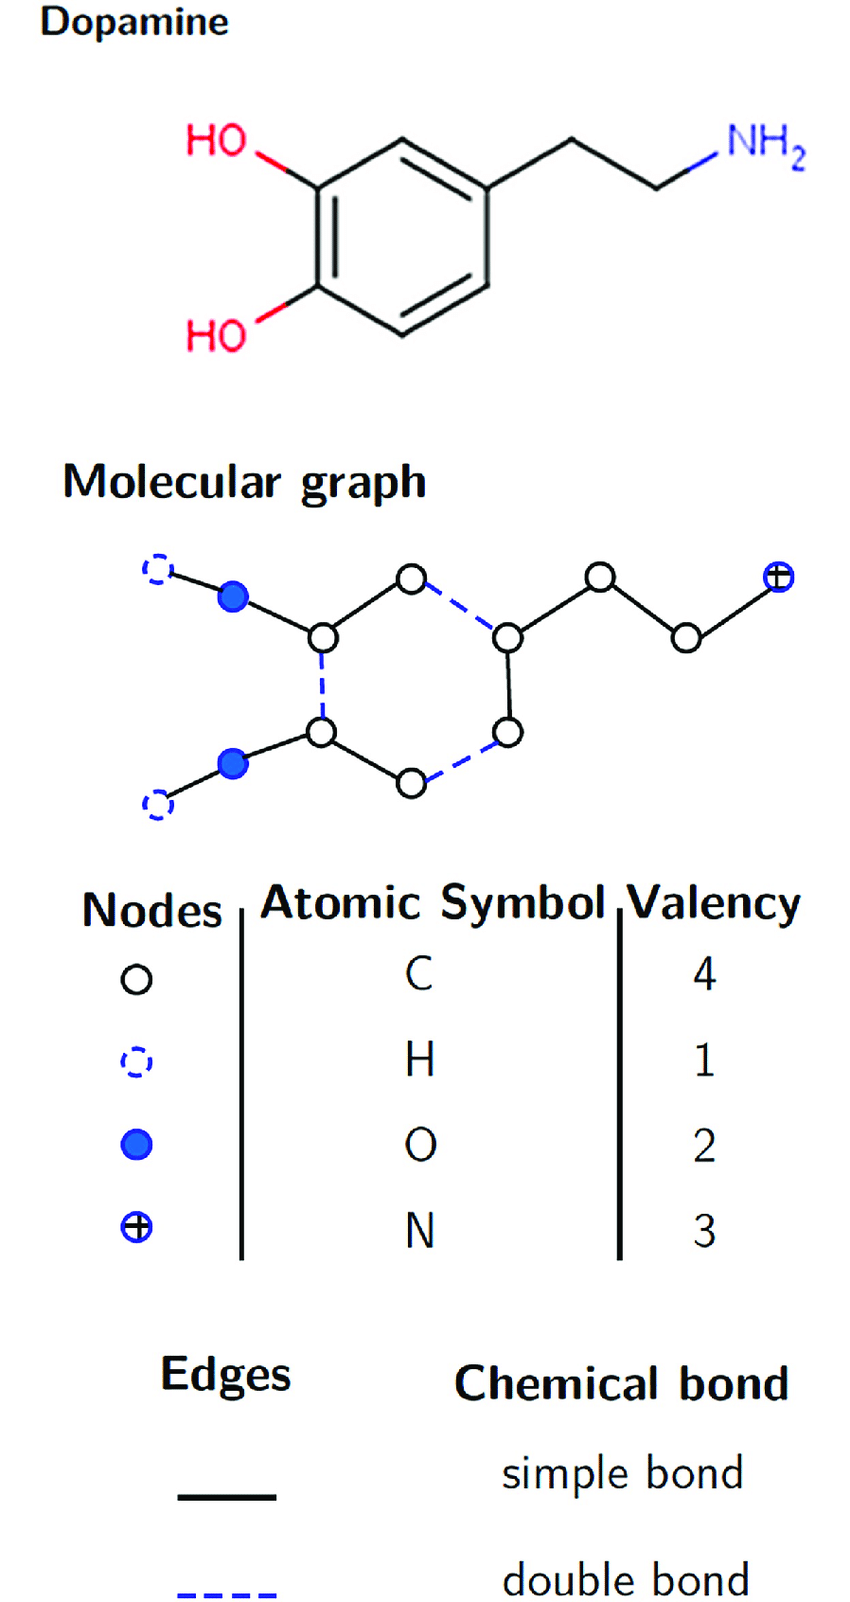
\includegraphics[width=0.5\textwidth]{Figures/chap_gnn/dopamine.png}
    \caption{Dopamine molecule represented as a graph. Different types of nodes represent different atoms and different edges represent the chemical bonds present in the molecule. Image source \citet{article:stefi}.}
    \label{fig:dopamine}
  \end{figure}
\item
  \textbf{Social Networks}. Social networks are networks between
    social actors who interact with each other. These types of networks
    are important when studying patterns of collective behaviour. In this
    representation, it is common to represent actors as nodes and their
    relationship as edges.
  
\end{itemize}


% The tasks that a GNN can be used to accomplish can be
% divided in three main categories, graph (or master) level, node level and edge level.
% All of these 
\begin{itemize}
\item
  \textbf{Graph-level task}. These types of tasks operate
  on the global (or master) node, and 
\end{itemize}